
\chapter{Introdução às Apresentações com LaTeX}
\label{ch:intro}

Este capítulo serve como uma porta de entrada para o mundo das apresentações criadas com LaTeX, uma poderosa ferramenta de tipografia e formatação. Ao explorar este tema, destacamos não apenas as vantagens, mas também as características únicas que diferenciam as apresentações LaTeX de outras plataformas. Ao utilizar LaTeX, os usuários desfrutam de um controle preciso sobre a estética e o layout de seus slides, permitindo uma personalização sem precedentes. Desde a escolha da tipografia até a configuração minuciosa dos elementos visuais, LaTeX oferece uma flexibilidade incomparável para a expressão criativa.

Além disso, este capítulo explora a integração harmoniosa de código em apresentações LaTeX, uma característica particularmente valiosa para aqueles que desejam incorporar elementos técnicos em suas apresentações. A capacidade de incluir trechos de código formatados de maneira elegante não apenas enriquece o conteúdo, mas também facilita a compreensão de conceitos complexos.

Ao compreender as vantagens e as possibilidades oferecidas pelo LaTeX para apresentações, os leitores serão preparados para explorar mais profundamente os tópicos abordados neste guia, que abrange desde noções básicas até técnicas avançadas de design de slides. Este capítulo serve como base sólida para a jornada que está por vir, fornecendo uma compreensão fundamental do potencial e da versatilidade das apresentações com LaTeX.

\section{Vantagens das Apresentações com LaTeX}
\label{sec:vantagens}

Quando se trata de criar apresentações visualmente atraentes e profissionais, o LaTeX oferece uma série de vantagens significativas em comparação com outras ferramentas de criação de slides disponíveis. Uma das principais vantagens é o controle preciso sobre a tipografia e o layout dos slides. Com LaTeX, os usuários podem personalizar cada elemento da apresentação, desde o tamanho e a fonte do texto até a posição e o estilo dos gráficos e imagens. Isso permite que os apresentadores criem slides que se destacam visualmente e comunicam efetivamente suas ideias.

Além disso, as apresentações LaTeX são altamente portáteis e compatíveis com uma variedade de dispositivos e plataformas. Os arquivos LaTeX podem ser facilmente compartilhados e visualizados em diferentes sistemas operacionais e dispositivos, garantindo uma experiência consistente para todos os espectadores. Isso é especialmente importante em ambientes profissionais e acadêmicos, onde a interoperabilidade e a acessibilidade são essenciais.

Outra vantagem significativa das apresentações LaTeX é a sua estabilidade e confiabilidade. Ao contrário de algumas ferramentas de criação de slides baseadas em software proprietário, o LaTeX é um sistema de código aberto amplamente utilizado e testado pela comunidade. Isso significa que os usuários podem confiar na consistência e na qualidade das apresentações produzidas com LaTeX, sem se preocupar com problemas de compatibilidade ou erros de formatação.



\begin{definition}
    LaTeX é um sistema de preparação de documentos de alta qualidade que oferece controle preciso sobre a tipografia e a formatação. Oferecendo uma combinação única de personalização, portabilidade e confiabilidade, tornando-as uma escolha ideal para profissionais e acadêmicos que desejam criar slides impactantes e eficazes.
\end{definition}

\section{Personalização e Flexibilidade}
\label{sec:personalizacao}

Uma das características distintivas do LaTeX para apresentações é sua excepcional capacidade de personalização e flexibilidade. Com LaTeX, os usuários têm controle total sobre cada elemento do slide, desde o layout até os detalhes mais sutis da formatação.

Por exemplo, ao criar um slide no LaTeX usando a classe Beamer, podemos facilmente personalizar o layout e adicionar conteúdo usando comandos específicos. Aqui está um exemplo simples de um slide que demonstra essa flexibilidade:

\begin{example}
    \begin{verbatim}
        \documentclass{beamer}
        \begin{document}
        \begin{frame}{Slide de Exemplo}
            \begin{itemize}
                \item Este é um item em uma lista.
                \item Este é outro item em uma lista.
            \end{itemize}
        \end{frame}
        \end{document}
    \end{verbatim}
\end{example}


Neste exemplo, estamos usando a classe Beamer para criar um slide simples com uma lista de itens. O comando begin{frame} inicia um novo slide, e o comando begin{itemize} cria uma lista com marcadores. Cada item da lista é especificado com o comando item.

Com os poucos comandos apresentados no Exemplo 1.1, somos capazes de gerar o seguinte resultado:
\begin{figure}[H]
    \centering
    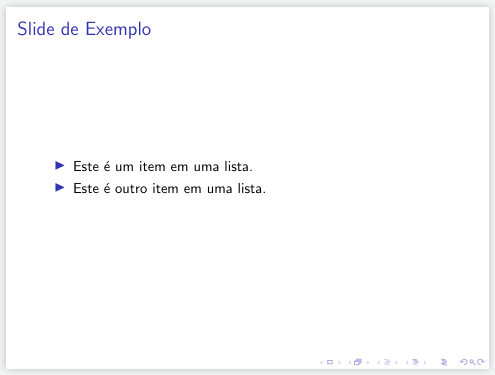
\includegraphics[width=0.5\linewidth]{images/exemplo1.1.png}
    \caption{Resultado do código do Exemplo 1.1}
    \label{fig:enter-label}
\end{figure}


Além disso, com LaTeX, podemos utilizar pacotes especializados para adicionar funcionalidades avançadas aos slides, como gráficos, tabelas e equações matemáticas. Essa versatilidade permite que os apresentadores criem apresentações que atendam às suas necessidades específicas e comuniquem suas ideias de forma clara e eficaz.

Portanto, a capacidade de personalização e flexibilidade oferecida pelo LaTeX é uma das razões pelas quais muitos profissionais e acadêmicos escolhem esta ferramenta para criar suas apresentações.



\subsection{Integração com Código}
\label{subsec:integracao}

A capacidade de integrar código diretamente nas apresentações é uma característica poderosa do LaTeX...

\begin{remark}
    Com LaTeX, é possível incluir trechos de código formatados de maneira elegante nos slides, facilitando a apresentação de projetos técnicos e demonstrações de software.
\end{remark}

\section{Desafios e Considerações}
\label{sec:desafios}

Embora as apresentações com LaTeX ofereçam muitos benefícios, também há desafios a serem considerados...

\begin{exercise}
    Considere os desafios de aprender LaTeX para criação de apresentações...
\end{exercise}

\begin{solution}
    A curva de aprendizado do LaTeX pode ser íngreme para iniciantes, mas existem recursos e comunidades online disponíveis para ajudar na aprendizagem...
\end{solution}